 \section{Mathematics Formulate}
 \label{Mathmatics}
    In order to get $N^{\prime}$, we consider $P_{s,i|N}$, which is the probability that an UE successfully performs its $i^{th}$ transmissions given $N$ users attempting to perform preamble transmissions, and the access success probability can be derived as
     \begin{eqnarray}
     \label{access success prob}
         P_{s,i|N}=p_{d,i}(\frac{R-1}{R})^{N-1},
     \end{eqnarray}
     where $p_{d,i}$ is the preamble detection probability applied to model the effect of path loss and power ramping, and it is shown in equation (\ref{preamble detection prob}). Moreover, equation (\ref{access success prob}) means that a UE succeeds in the $i^{th}$ preamble transmission if all the other $N - 1$ UEs select the other $R - 1$ preambles, and the non-collided preamble is detected by the eNB.
     \begin{eqnarray}
     \label{preamble detection prob}
         p_{d,i} = 1 - (\frac{1}{e})^i
     \end{eqnarray}
     Let $N_s$ be the number of UEs who successfully perform preamble transmissions. As a result, we consider $E(N_s|N)$ as the the expected number of UEs who successfully perform preamble transmission given N users attempting to perform preamble transmissions, and the $E(N_s|N)$ is given by
     \begin{align}
     \label{exp devices}
         E{(N_s|N)}&=\sum_{i=1}^{\theta}N_i P_{s,i|N} \notag \\
         &=\sum_{i=1}^{\theta}N_i p_{d,i} (\frac{R-1}{R})^{N-1} \notag \\
         &=\frac{\sum_{i=1}^{\theta}  N_i p_{d,i}}{N} N (\frac{R-1}{R})^{N-1} \notag \\
         &=\bar{p_d} N (\frac{R-1}{R})^{N-1},
     \end{align}
    \begin{figure}[t]
    \centering
    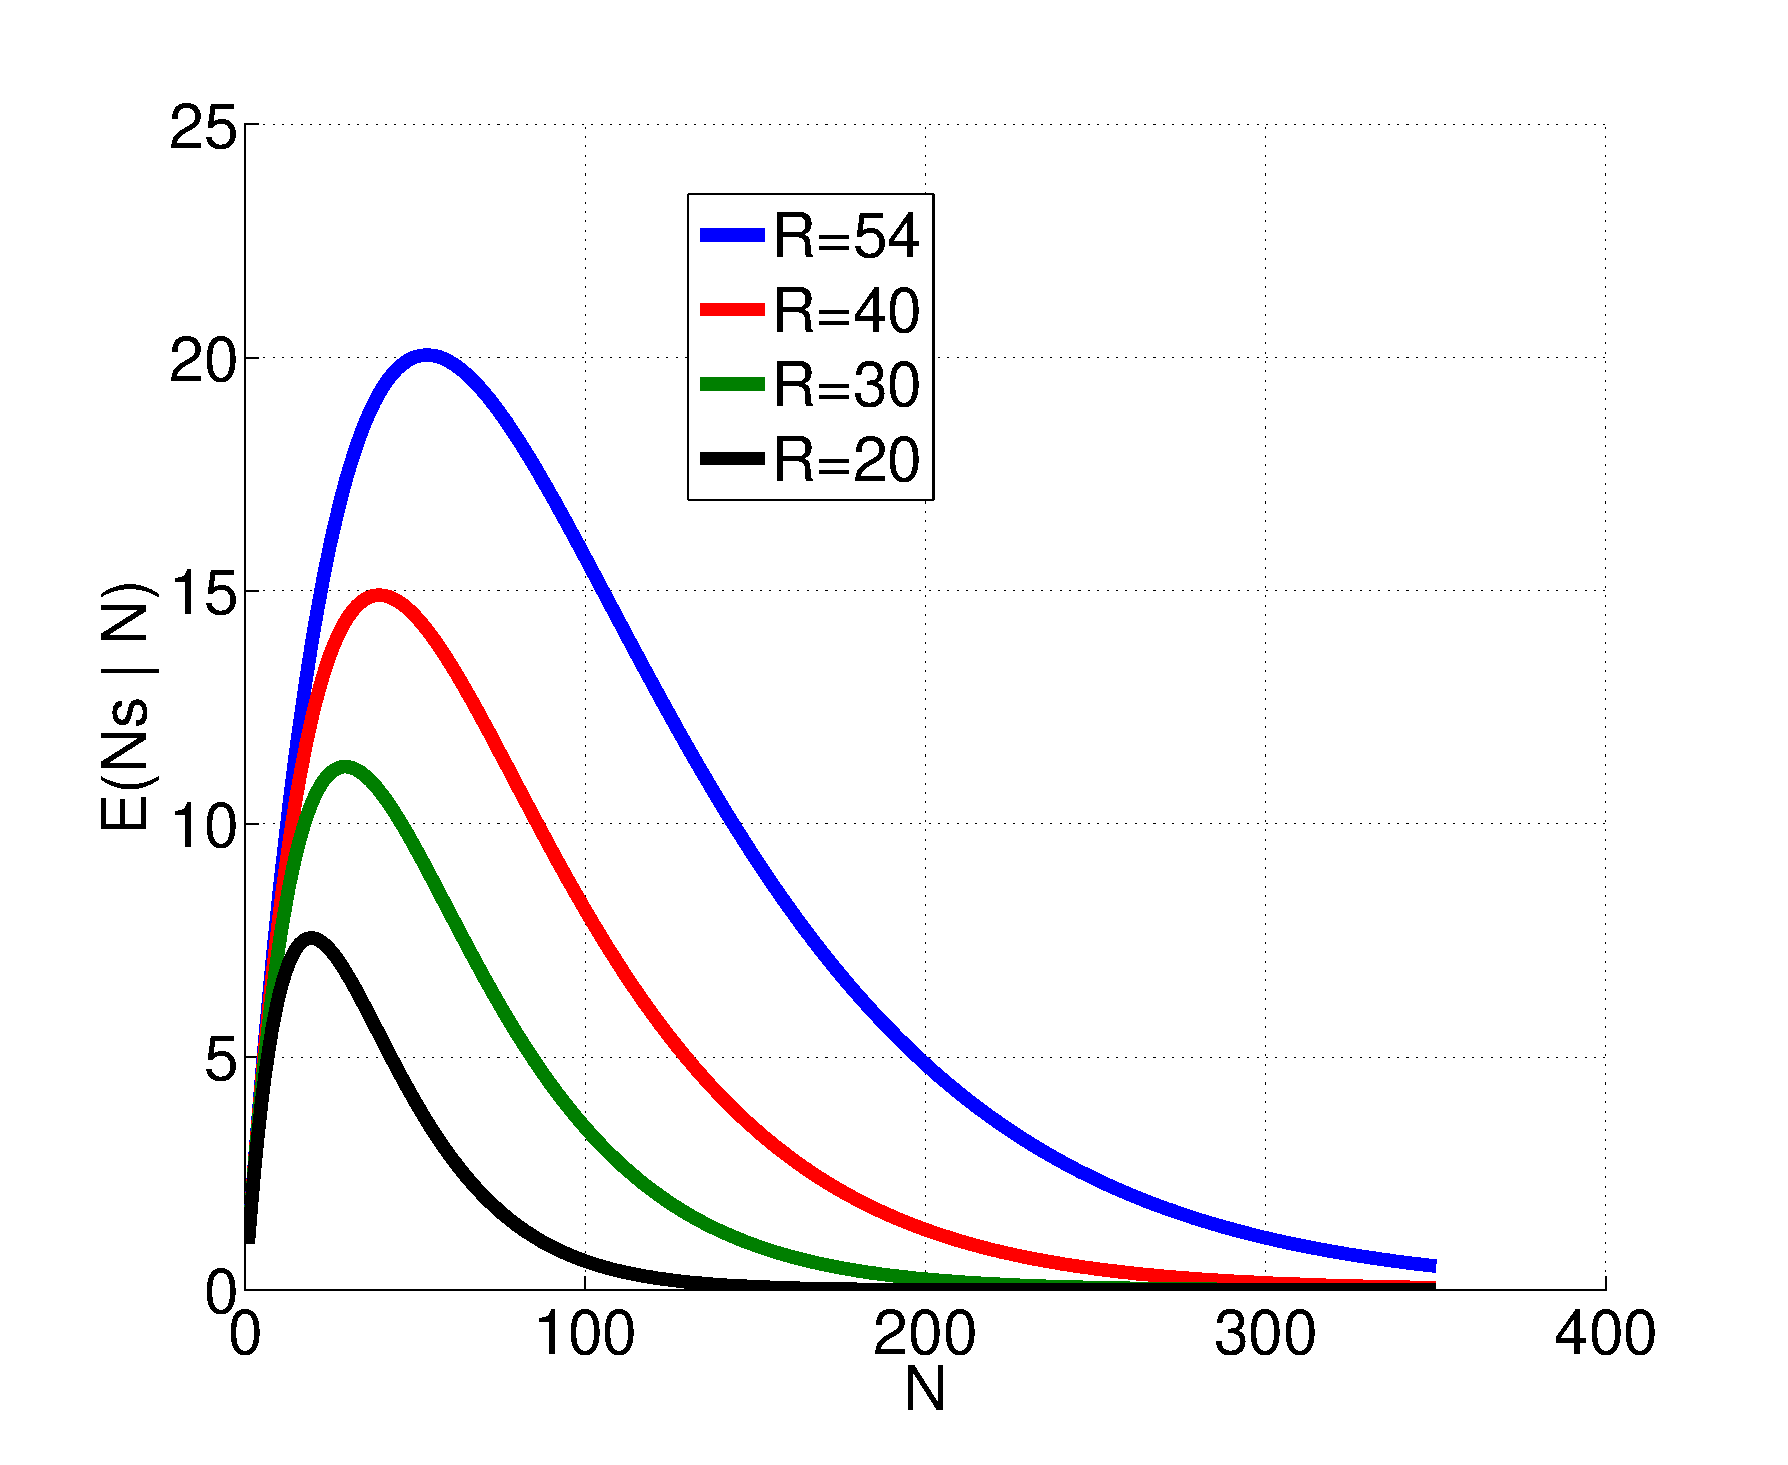
\includegraphics[width=3.8in]{fig_exp_suc_UE.eps}
    \caption{The expected number of success UEs}
    \label{fig_exp_suc_UE}
    \end{figure}
     where $\theta$ is the maximum number of preamble transmissions and $\bar{p_d}$ is the expected preamble detection probability (e.g., $\bar{p_d} = \frac{\sum_{i=1}^{\theta} N_i^j p_{d,i}}{\sum_{i=1}^{\theta}N_i^j}$, where $\sum_{i=1}^{\theta}N_i^j=N^j$). We can get the expectation of UEs who successfully perform preamble transmissions given $\bar{p_d}=1 $ (ideal condition) according to the variation of $N$ in Fig.~\ref{fig_exp_suc_UE}, and the equation (\ref{exp devices}) is also mentioned in~\cite{lin2015estimation}.%推得與reference相同的式子

     %利用不同的N在理想的情況下 Pd bar=1 可得到的對應成功人數期望值的upper bound

     Due to the reason that we cannot get the closed form solution of $N$ in equation (\ref{exp devices}), we propose a new method to get $N^\prime$, which is the estimation of $N$. At first, we have to compute the $\bar{p_d}$, but the bottleneck is that eNB cannot know the total number of UEs who perform $i^{th}$ preamble transmission in an RACH slot. In other words, if the $N^j_i$ is unknown, $\bar{p_d}$ cannot be derived. In order to solve the problem, we use the existing message which can be obtained by eNB to derive the $\bar{p_d}^\prime$, which is the approximation of $\bar{p_d}$. Therefore, we consider $N_{s,i}$ as the substitute of $N$, so the $\bar{p_d}^\prime$ can be derived as
     \begin{align}
         \bar{p_{d}}^\prime = \frac{\sum_{i=1}^{\theta} N_{s,i} p_{d,i} }{\sum_{i=1}^{\theta}{N_{s,i}}},
     \end{align}

    % \begin{figure}[t]
    % \centering
    % 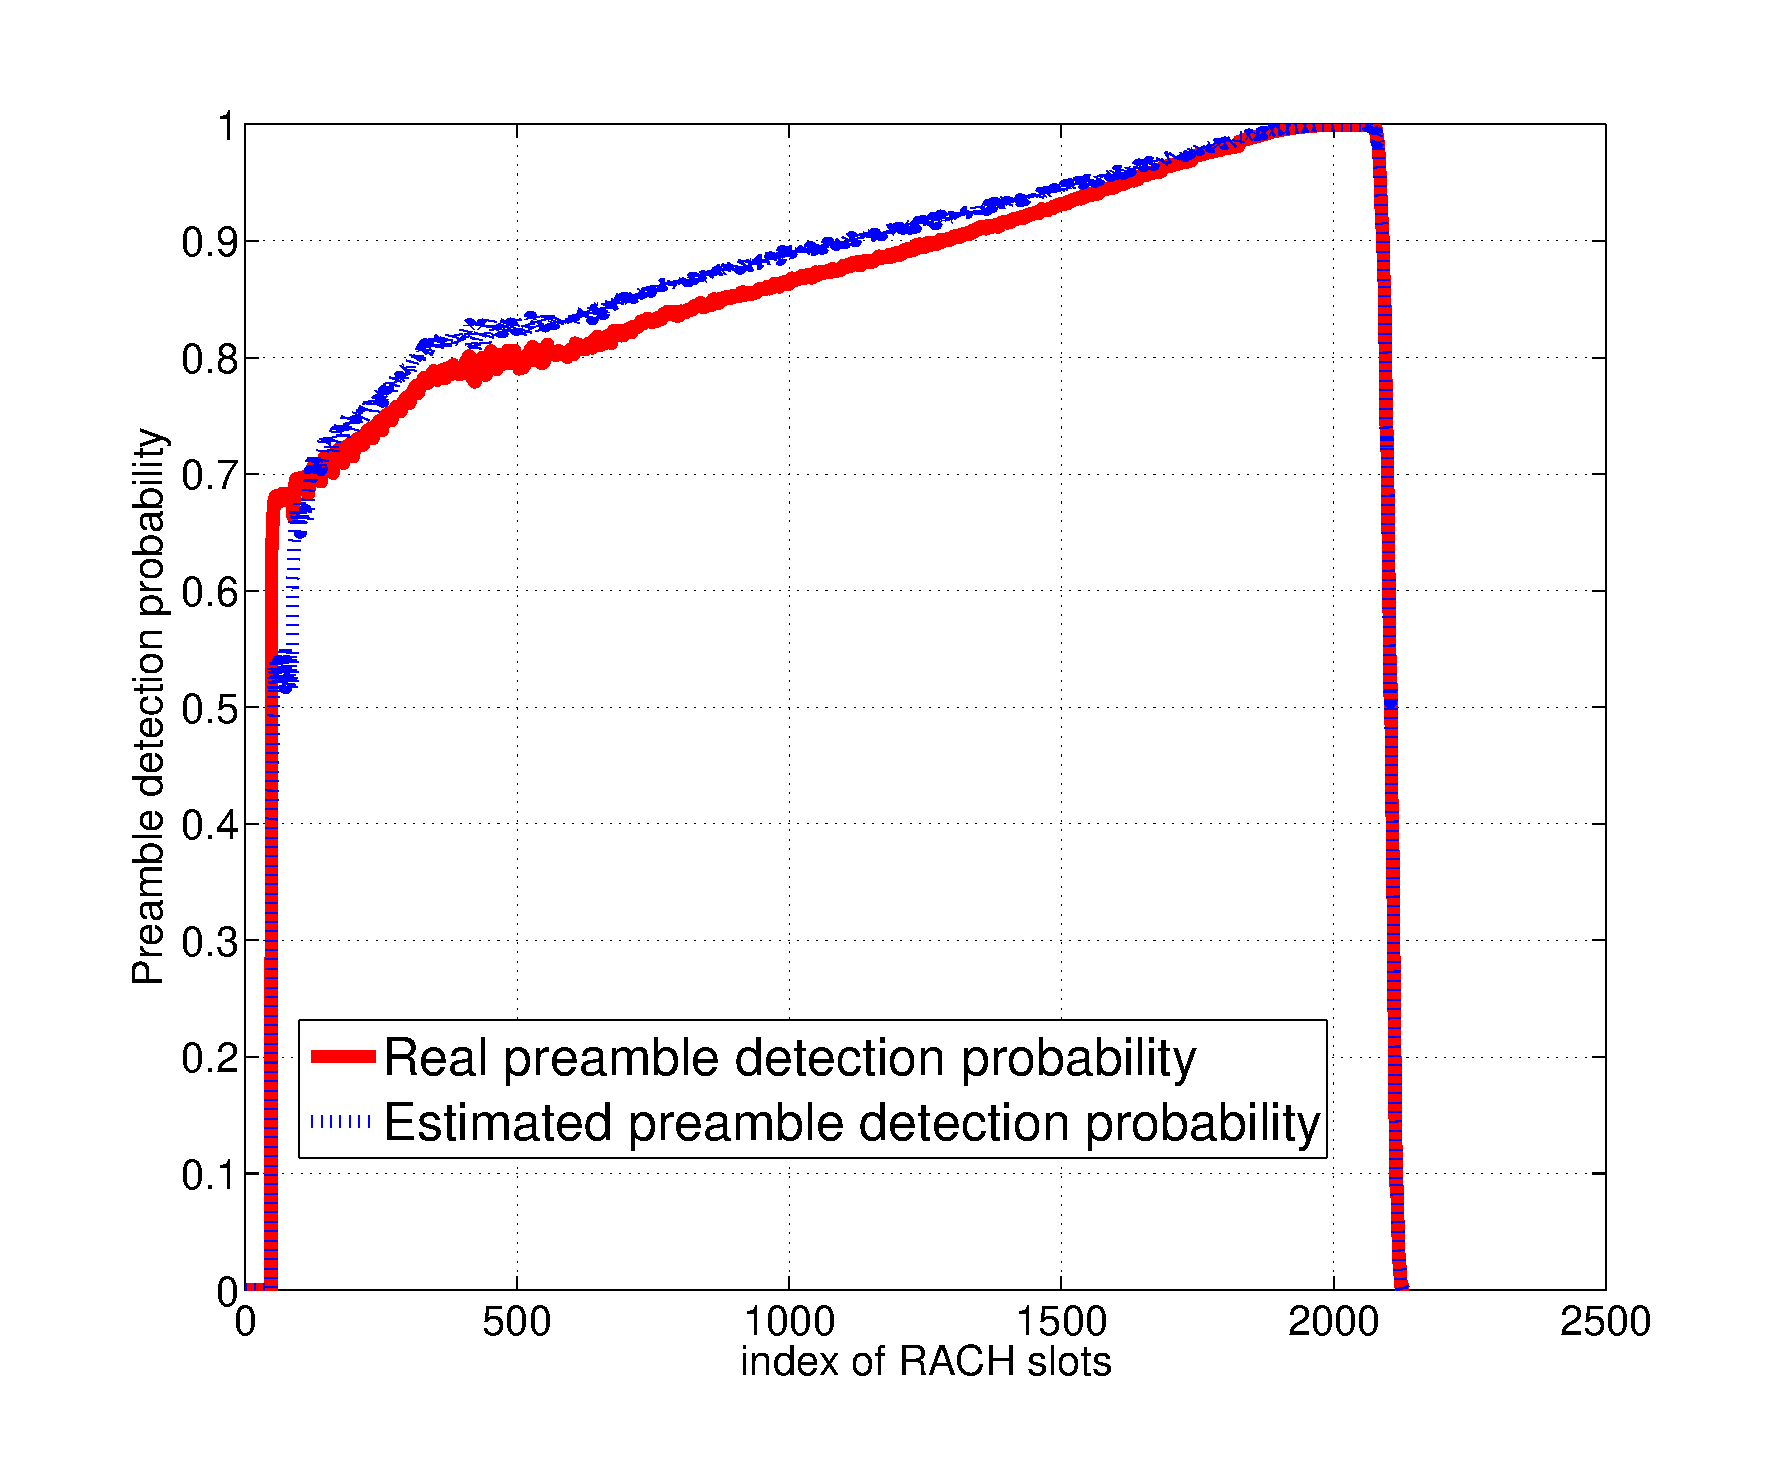
\includegraphics[width=3.8in]{fig_pd_compare.eps}
    % \caption{Comparison between $\bar{p_d}$ and $\bar{p_d}^{\prime}$}
    % \label{fig_pd_compare}
    % \end{figure}

    \begin{figure}[t]
    \centering
    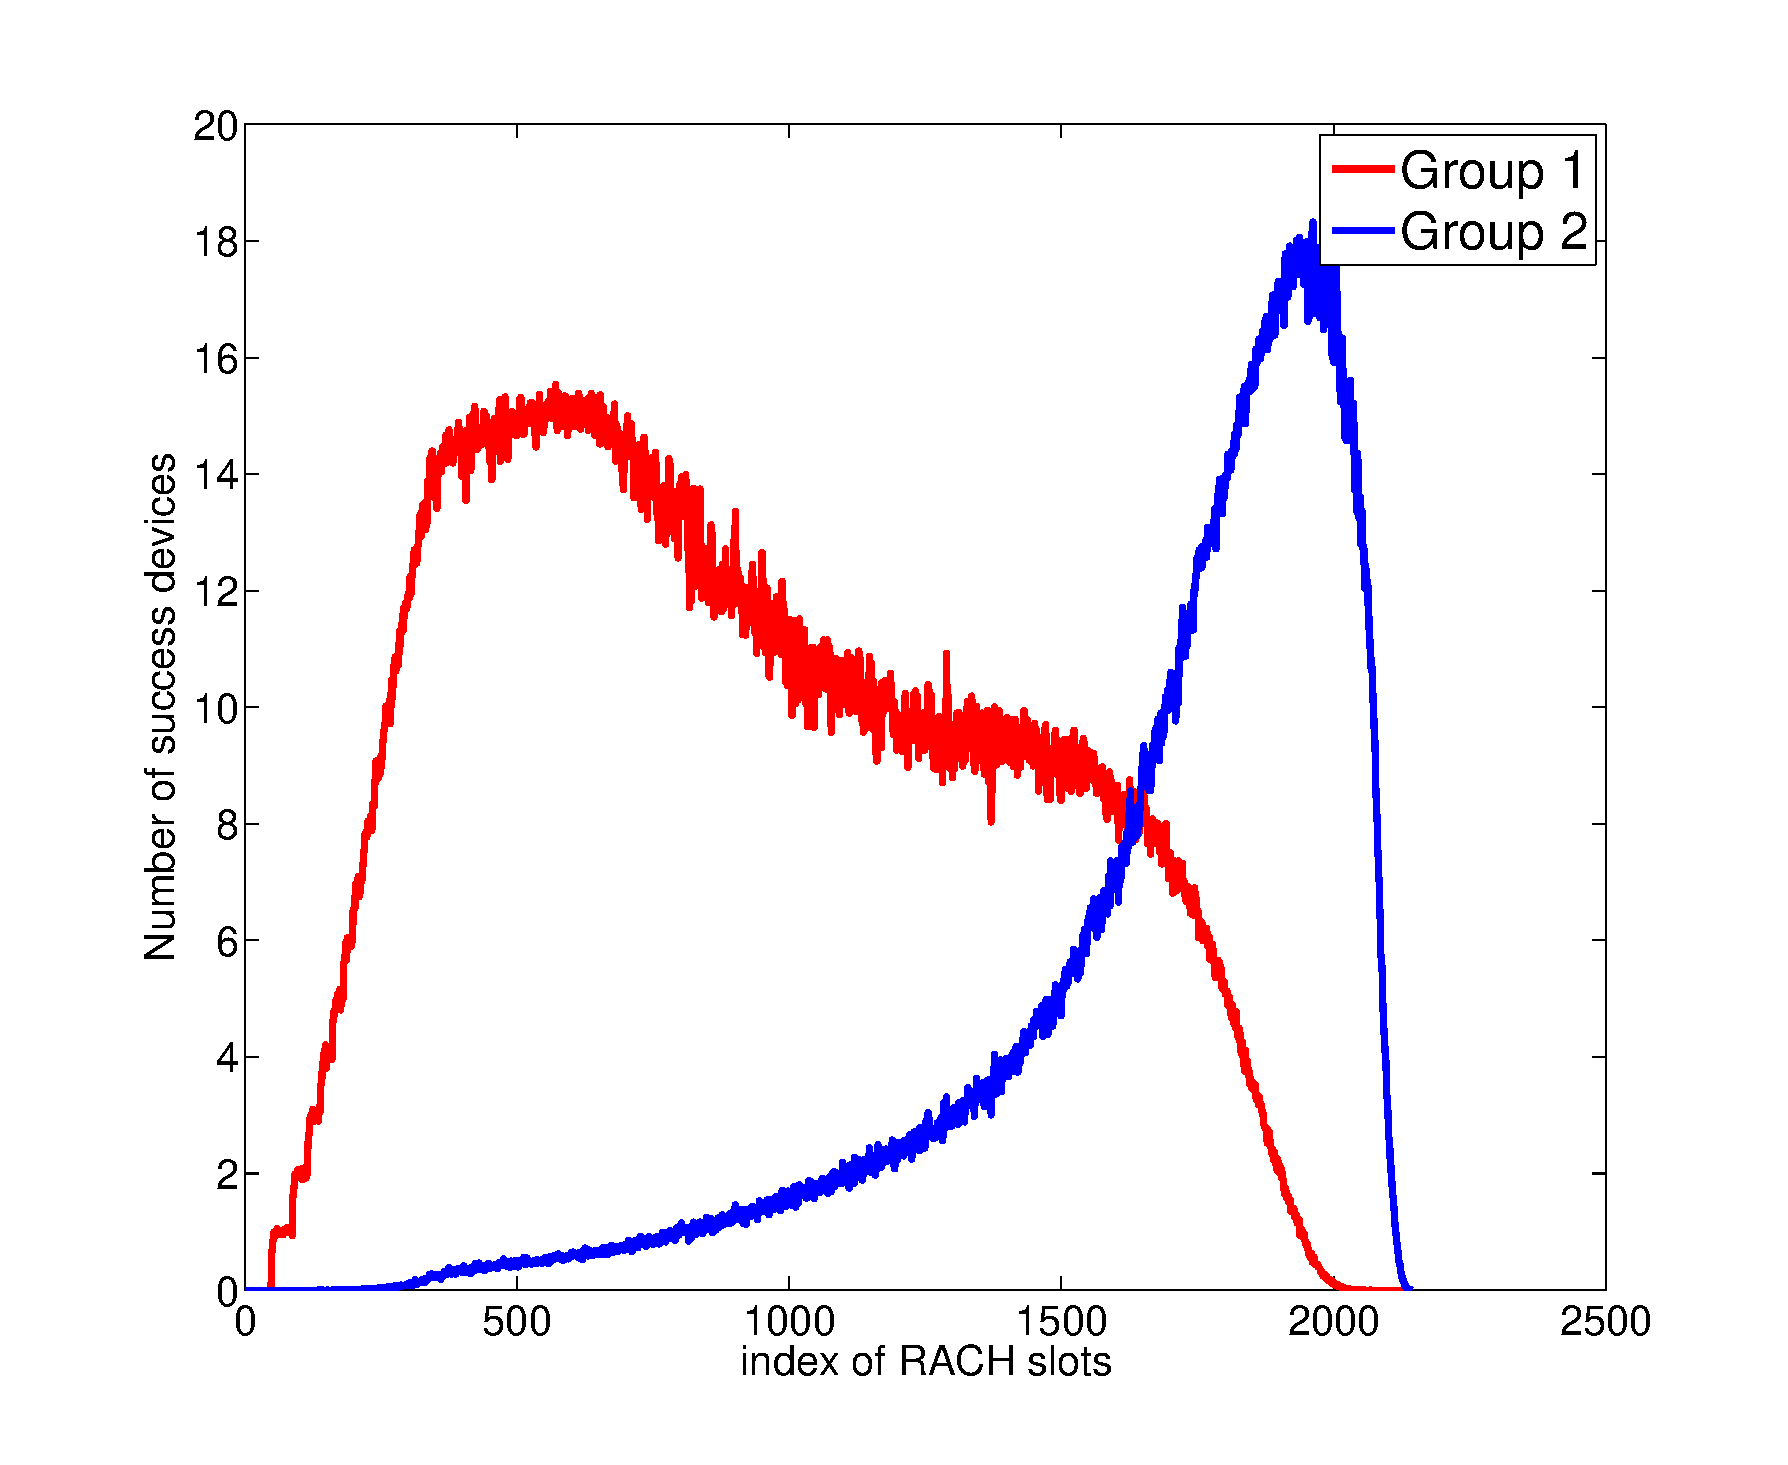
\includegraphics[width=3.8in]{fig_propose_suc_gorup.eps}
    \caption{Number of success devices in each group}
    \label{fig_propose_suc_group}
    \end{figure}
     where the $N_{s,i}$ is the number of success UEs who successfully perform $i^{th}$ preamble transmission in an RACH slot. Although $\bar{p_{d}}^\prime$ maybe not true approximate $\bar{p_d}$ in certain condition, it will be more closed to $\bar{p_d}$ when congestion condition happens. When the congestion happens, UE will try to perform random access procedure again until the $RetryCounter$ is larger than the maximum preamble transmissions. As mentioned above, the number of UEs, whose $RetryCounter$ are close to the maximum preamble transmissions, increases rapidly shown in Fig.~\ref{fig_propose_suc_group}, and it may cause that both of the $\bar{p_d}$ and $\bar{p_d}^\prime$ approximate to $1$. In short, $\bar{p_d}^\prime$ can be used to detect congestion sensitively so that we can make a change immediately.

    %在已知成功人數、推測的Pd bar prime和可用的preamble數之後,我們就可以從現實狀況的成功人數推測到理想狀況的成功人數,藉此求得未知total的總人數
     Upon deriving the $\bar{p_d}^\prime$ which is used to replace of the $\bar{p_d}$, we make a transposition of $\bar{p_d}^\prime$ in equation (\ref{exp devices}), and the modified equation is shown as follows.
     \begin{align}
     \label{est function}
         \frac{E{(N_s|N)}}{\bar{p_{d}}^\prime} = N (\frac{R-1}{R})^{N-1}
     \end{align}

     With the equation (\ref{est function}), we have $\frac{E{(N_s|N)}}{\bar{p_{d}}^\prime}$, which is new expected number of success UEs in ideal condition, to estimate $N^\prime$ through the look-up table in Fig.~\ref{fig_exp_suc_UE}.

    \subsection{eNB Updates the ACB Barring Factor Dynamically}
    \begin{algorithm}
      \caption{Update ACB Barring Factor Dynamically without congestion control}
        \begin{algorithmic}[1]
        \State input: $R$, number of success preambles and collision preambles, design parameters $w_m$
        \State set $time\ slot=0$; $p_m=1$, for all $m$
        \While $\ N_s+N_f<N$
        \State $time\ slot= time\ slot + 1$;
         \If {(activate preamble $\geq 50$ percent )}
         \State check the table and then set $\max(N^\prime)$
          \Else
          \State check the table and then set $\min(N^\prime)$
                   \State $W=\{w_1,w_2,..,w_m\}$, sort $W$ to an descending order
                   \State set $w^\prime = m^{th}$ weight in set $W$
                   \State $p_{m}=\frac{w^\prime R}{N^\prime};$
            \EndIf
          \EndWhile
          \end{algorithmic}
     \end{algorithm}
%%%%%%%%%%%%%%%%%%%%%%%%%%%%%%%%%%%%%%%%%%%%%%%%%%%%%%%%%%%%%%%%%%%%%%%%%%%%%%%%%%%%%%%%%%%%%%%%%%%%

     \begin{algorithm}
      \caption{Update ACB Barring Factor Dynamically with congestion control}
        \begin{algorithmic}[1]
        \State input: $R$, number of success preambles and collision preambles, design parameters $w_m$
        \State set $time\ slot=0$; $p_m=1$, for all $m$
        \While $\ N_s+N_f<N$
        \State $time\ slot= time\ slot + 1$;
         \If {(activate preamble $\geq 50$ percent )}
         \State check the table and then set $\max(N^\prime)$
          \Else
          \State check the table and then set $\min(N^\prime)$ \\
                \If{(number of success transmitted preambles $\leq 0.2 *$ number of activate preambles)}\\
                \%{Congestion Control}
                   \State $W=\{w_1,w_2,..,w_m\}$, sort $W$ to an descending order
                   \State set $w^\prime = m^{th}$ weight in set $W$
                   \State $p_{m}=\frac{w^\prime R}{N^\prime};$
                \Else \\
                \%{No congestion Control}
                   \State $W=\{w_1,w_2,..,w_m\}$, sort $W$ to a ascending order
                   \State set $w^\prime = m^{th}$ weight in set $W$
                   \State $p_{m}=\frac{w^\prime R}{N^\prime};$
                \EndIf
            \EndIf
          \EndWhile
          \end{algorithmic}
     \end{algorithm}
 %%%
    Each group, whose threshold (number of preamble transmissions) is larger than other groups, has higher priority and index. Therefore, we assign each group to a different weight, and the groups with higher priority are assigned to a larger weight. The weight of group $m$, $w_m$, can be considered as the the proportion of the allocation of RACH resources, so it should be defined as $\sum_{m=1} w_m=1$. We follow the example of Fig.~\ref{fig_broadcast_groups} to divide MTC devices into two groups, and the weight of group $2$ is higher than group $1$ (e.g., $w_2>w_1$) due to we hope the groups whose number of preamble transmissions close to maximum preamble transmissions; So that group $2$ can own more RACH resources to promote the access success probability.

    We aim at distributing MTC devices over several RACH slots when congestion happens. The maximal $E(N_s|N)$ is achieved by setting $N$ equal to $R$ or $R-1$ as illustrated in Fig.~\ref{fig_exp_suc_UE}. In other words, we hope that there are only $N\approx R$ MTC devices who attempt to perform preamble transmission in an RACH slot, so it can be derived as
    \begin{align}
    \label{ACB_factor}
      \sum_{m=1}^{n} N^\prime p_m=\sum_{m=1}^{n}w_mR=R,
    \end{align}
    where the $p_m$ is the ACB factor of group $m$ and the $R_m$ is the number of MTC devices who belong to group $m$ and pass the ACB scheme. Thus, the $p_m$ which is the ACB factor of group $m$ is able to be obtained from equation (\ref{ACB_factor}) shown in the following.
    \begin{align}
      p_m=\frac{W_m R}{N^\prime}
    \end{align}

    Our algorithm to adjust ACB parameter $p$ is shown in Algorithm 1 and 2. In these two algorithms, we take the preamble utility into account because it can reflect the number of MTC devices who attempt to perform preamble transmissions indirectly. When there are two possible $N^\prime$ after inquiring the Fig.~\ref{fig_exp_suc_UE}, it is determined by the preamble utility. If the preamble utility is low, we set the smaller one of the $N^\prime$. Otherwise, if the preamble utility is high, we choose the larger $N^\prime$ to be the estimation of $N$. 
    In Algorithm 2, eNB confirms whether the number of success preambles is less or equal to the $20$ percent of the number of activate preambles at each time slot. If it is, the group which has the $m^{th}$ highest priority will be assigned the $m^{th}$ weight from the set $W$ which is an descending order. If it is not, the group which has the $m^{th}$ highest priority will be assigned the $m^{th}$ weight from the set $W$ which is an ascending order. 